\documentclass{article}%
\usepackage[T1]{fontenc}%
\usepackage[utf8]{inputenc}%
\usepackage{lmodern}%
\usepackage{textcomp}%
\usepackage{lastpage}%
\usepackage{geometry}%
\geometry{left=2.5cm,top=1.5cm}%
\usepackage[dvipsnames]{xcolor}%
\usepackage{graphicx}%
\usepackage{array}%
\usepackage{colortbl}%
\usepackage{caption}%
\usepackage{slashbox}%
\usepackage{amsmath}%
\usepackage{xcolor}%
\usepackage{multirow}%
\usepackage{tcolorbox}%
\usepackage{booktabs}%
\usepackage{ragged2e}%
%
\graphicspath{ {D:/CARPETAS W10/Escritorio/GITHUB/automatizacion_estructural/} }%
%
\begin{document}%
\normalsize%
\subsection{Factor de Zona}%
\label{subsec:FactordeZona}%
%


\begin{table}[ht!]%
\begin{minipage}{0.55\textwidth}%
\caption{Factor de zona}%
\begin{tabular}{|>{\centering\arraybackslash}m{3.75cm}|>{\centering\arraybackslash}m{3.75cm}|}%
\hline%
\multicolumn{2}{|c|}{\textbf{FACTOR DE ZONA SEGÚN E{-}030}}\\%
\hline%
\textbf{ZONA}&\textbf{Z}\\%
\hline%
<<<<<<< HEAD
Zona&Z\\%
=======
4\cellcolor[rgb]{ .949,  .949,  .949} &\textcolor[rgb]{ 1,  0,  0}{\textbf{0.45}}\cellcolor[rgb]{ .949,  .949,  .949} \\%
\hline%
3&0.35\\%
\hline%
2&0.25\\%
\hline%
1&0.10\\%
>>>>>>> main
\hline%
\end{tabular}%
\end{minipage}%
\begin{minipage}{0.35\textwidth}%
\begin{center}%
\includegraphics[width=4cm]{mapa_zona}%
\end{center}%
\end{minipage}%
\caption*{Fuente: E-30 (2018)}%
\end{table}

%
\subsubsection{Factor de suelo}%
\label{ssubsec:Factordesuelo}%
%


\begin{table}[ht!]%
\centering%
\caption{Factor de zona}%
\begin{tabular}{|>{\centering\arraybackslash}m{3.75cm}|>{\centering\arraybackslash}m{2cm}|>{\centering\arraybackslash}m{2cm}|>{\centering\arraybackslash}m{2cm}|>{\centering\arraybackslash}m{2cm}|}%
\hline%
\multicolumn{5}{|c|}{\textbf{FACTOR DE SUELO SEGÚN E{-}030}}\\%
\hline%
\backslashbox{\textit{\textbf{ZONA}}}{\textit{\textbf{SUELO}}}&\textbf{S0}&\textbf{S1}&\textbf{S2}&\textbf{S3}\\%
\hline%
4\cellcolor[rgb]{ .949,  .949,  .949} &0.80\cellcolor[rgb]{ .949,  .949,  .949} &1.00\cellcolor[rgb]{ .949,  .949,  .949} &\textcolor[rgb]{ 1,  0,  0}{\textbf{1.05}}\cellcolor[rgb]{ .949,  .949,  .949} \cellcolor[rgb]{ .949,  .949,  .949} &1.10\cellcolor[rgb]{ .949,  .949,  .949} \\%
\hline%
3&0.80&1.00&1.15\cellcolor[rgb]{ .949,  .949,  .949} &1.20\\%
\hline%
2&0.80&1.00&1.20\cellcolor[rgb]{ .949,  .949,  .949} &1.40\\%
\hline%
1&0.80&1.00&1.60\cellcolor[rgb]{ .949,  .949,  .949} &2.00\\%
\hline%
\end{tabular}%
\caption*{Fuente: E-30 (2018)}%
\end{table}

%
\subsubsection{Periodos de suelo}%
\label{ssubsec:Periodosdesuelo}%
%


\begin{table}[ht!]%
\centering%
\caption{Periodos de suelo}%
\begin{tabular}{|>{\centering\arraybackslash} m{2cm}|>{\centering\arraybackslash}m{2cm}|>{\centering\arraybackslash}m{2cm}|>{\centering\arraybackslash}m{2cm}|>{\centering\arraybackslash}m{2cm}|}%
\cline{2-5}%
\multicolumn{1}{r|}{}&\multicolumn{4}{c|}{\textbf{PERIODO "Tp" y "Tl" SEGÚN E-030}}\\%
\cline{2-5}%
\multicolumn{1}{r|}{}&\multicolumn{4}{c|}{\textit{\textbf{Perfil de suelo}}}\\%
\cline{2-5}%
\multicolumn{1}{r|}{}&\textbf{S0}&\textbf{S1}&\textbf{S2}&\textbf{S3}\\%
\hline%
Tp&0.30&0.40&\textcolor[rgb]{ 1,  0,  0}{\textbf{0.60}}\cellcolor[rgb]{ .949,  .949,  .949} &1.00\\%
\hline%
Tl&3.00&2.50&\textcolor[rgb]{ 1,  0,  0}{\textbf{2.00}}\cellcolor[rgb]{ .949,  .949,  .949} &1.60\\%
\hline%
\end{tabular}%
\caption*{Fuente: E-30 (2018)}%
\end{table}

%
\subsubsection{Sistema Estructural}%
\label{ssubsec:SistemaEstructural}%
<<<<<<< HEAD
Después de realizar el análisis sísmico se determino que los sistemas estructurales en X, Y son:%
%
=======
Después de realizar el análisis sísmico se determino que los sistemas estructurales en X, Y son %
Pórticos de Concreto Armado y Dual de Concreto Armado respectivamente%
%insertion%
>>>>>>> main


\begin{table}[ht!]%
\caption{coeficiente básico de reducción}%
\begin{tabular}{|>{\arraybackslash}m{10cm}| >{\centering\arraybackslash}m{4cm}|}%
\hline%
\multicolumn{2}{|c|}{\textbf{SISTEMAS ESTRUCTURALES}}\\%
\hline%
\textbf{Sistema Estructural}&\multicolumn{1}{m{4cm}|}{\textbf{Coeficiente Básico de Reducción Ro}}\\%
\hline%
\multicolumn{2}{|l|}{\textbf{Acero:}}\\%
\hline%
Porticos Especiales Resistentes a Momento (SMF)&8\\%
\hline%
Porticos Intermedios Resistentes a Momento (IMF)&5\\%
\hline%
Porticos Ordinarios Resistentes a Momento (OMF)&4\\%
\hline%
Porticos Ordinarios Resistentes a Momento (OMF)&7\\%
\hline%
Porticos Ordinarios Concentricamente Arrriostrados (OCBF)&4\\%
\hline%
Porticos Excentricamente Arriostrados (EBF)&8\\%
\hline%
\multicolumn{2}{|l|}{\textbf{Concreto Armado:}}\\%
\hline%
Porticos\cellcolor[rgb]{ .949,  .949,  .949} &\textcolor[rgb]{ 1,  0,  0}{\textbf{8}}\cellcolor[rgb]{ .949,  .949,  .949} \\%
\hline%
<<<<<<< HEAD
Dual&7\\%
=======
Dual\cellcolor[rgb]{ .949,  .949,  .949} &\textcolor[rgb]{ 1,  0,  0}{\textbf{7}}\cellcolor[rgb]{ .949,  .949,  .949} \\%
>>>>>>> main
\hline%
De muros estructurales&6\\%
\hline%
Muros de ductilidad limitada&4\\%
\hline%
\textbf{Albañilería Armada o Confinada}&3\\%
\hline%
\textbf{Madera}&7\\%
\hline%
\end{tabular}%
\caption*{Fuente: E-30 (2018)}%
\end{table}

%
\subsubsection{Factor de Amplificación sísmica}%
\label{ssubsec:FactordeAmplificacinssmica}%
%
Se determina según el artículo 11 de la E{-}30%
\setlength{\jot}{0.5cm}%


\begin{figure}[h!]%
\caption{Factor de amplificación}%
\begin{minipage}{0.5\textwidth}%

    \begin{align*}
        &T< T_{P}         &   C&=2,5\cdot\left ( \frac{T_{P}}{T} \right )\\
        &T_{P}< T< T_{L}  &   C&=2,5\cdot\left ( \frac{T_{P}}{T} \right )\\
        &T> T_{L}         &   C&=2,5\cdot\left ( \frac{T_{P}\;T_{L}}{T^{2}} \right )
    \end{align*}%
\end{minipage}%
\begin{minipage}{0.4\textwidth}%
\centering%
\includegraphics[width=6.5cm]{Amplificacion}%
\end{minipage}%
\caption*{Fuente: Muñoz (2020)}%
\end{figure}

%
\subsubsection{Factor de Importancia}%
\label{ssubsec:FactordeImportancia}%
%


\begin{table}[h!]%
\centering%
\caption{Factor de Uso o Importancia}%
\begin{tabular}{|>{\arraybackslash}m{3cm}|m{8cm}|>{\arraybackslash}m{2.8cm}|}%
\hline%
\multicolumn{3}{|c|}{\textbf{CATEGORIA DE LA EDIFICACION}}\\%
\hline%
\multicolumn{1}{|c|}{\textbf{CATEGORIA}}&\multicolumn{1}{|c|}{\textbf{DESCRIPCION}}&\multicolumn{1}{|c|}{\textbf{FACTOR U}}\\%
\hline%
\multirow{2}[4]{3cm}{A Edificaciones Escenciales}&A1: Establecimiento del sector salud (públicos y privados) del segundo y tercer nivel, según lo normado por el ministerio de salud.&\multicolumn{1}{>{\centering\arraybackslash}m{2.8cm}|}{Con aislamiento 1.0 y sin aislamiento 1.5.}\\%
\cline{2-3}%
&A2: Edificaciones escenciales para el manejo de las emergencias, el funcionamiento del gobierno y en general aquellas que puedan servir de refugio después de un desastre.\cellcolor[rgb]{1,  .949,  .8}&\multicolumn{1}{>{\centering\arraybackslash}m{2.8cm}|}{\textcolor[rgb]{ 1,  0,  0}{\textbf{1.50}}\cellcolor[rgb]{1,  .949,  .8}}\\%
\hline%
B Edificaciones Importantes &Edificaciones donde se reúnen gran cantidad de personas tales como cines, teatros, estadios, coliseos, centros comerciales, terminales de buses de pasajeros, establecimientos penitenciarios, o que guardan patrimonios valiosos como museos y bibliotecas.&\multicolumn{1}{>{\centering\arraybackslash}m{2.8cm}|}{1.30}\\%
\hline%
C Edificaciones Comunes&Edificaciones comunes tales como: viviendas, oficinas, hoteles, restaurantes, depósitos e instalaciones industriales cuya falla no acarree peligros adicionales de incendios o fugas de contaminantes.&\multicolumn{1}{>{\centering\arraybackslash}m{2.8cm}|}{1.00}\\%
\hline%
D Edificaciones temporales&Construcciones provisionales para depósitos, casetas y otras similares.&\multicolumn{1}{>{\centering\arraybackslash}m{2.8cm}|}{A criterio del proyectista}\\%
\hline%
\end{tabular}%
<<<<<<< HEAD
\caption*{Fuente: E-30 (2018)}%
=======
\caption*{Fuente: E-030 (2018)}%
\end{table}

%
\subsubsection{Tabla resumen de parámetros sísmicos}%
\label{ssubsec:Tablaresumendeparmetrosssmicos}%
%insertion%


\begin{table}[H]%
\centering%
\caption{Resumen de parámetros sísmicos}%
\extrarowheight = -0.3ex%
\renewcommand{\arraystretch}{1.5}%
\begin{tabular}{m{5cm}|>{\centering\arraybackslash}m{2cm}|>{\centering\arraybackslash}m{2cm}|>{\centering\arraybackslash}m{2cm}|}%
\cline{2%
-%
4}%
&\multicolumn{3}{c|}{\textbf{PARÁMETROS SÍSMICOS}}\\%
\cline{2%
-%
4}%
\textit{\textbf{Norma E.030}}&&\textit{\textbf{X}}&\textit{\textbf{Y}}\\%
\cline{2%
-%
4}%
\textit{Factor de Zona (Tabla N° 1)}&\textbf{Z}&\multicolumn{2}{c|}{0.45}\\%
\cline{2%
-%
4}%
\textit{Factor de Uso (Tabla N° 5)}&\textbf{U}&\multicolumn{2}{c|}{1.50}\\%
\cline{2%
-%
4}%
\textit{Factor de Suelo (Tabla N° 3)}&\textbf{S}&\multicolumn{2}{c|}{1.05}\\%
\cline{2%
-%
4}%
\multirow{2}{*}{\textit{Periodos(Tabla N° 4)}}&\textbf{T\raisebox{-0.5ex}{\scriptsize{P}}}&\multicolumn{2}{c|}{0.60}\\%
\cline{2%
-%
4}%
&\textbf{T\raisebox{-0.5ex}{\scriptsize{L}}}&\multicolumn{2}{c|}{2.00}\\%
\cline{2%
-%
4}%
\textit{Coef. Básico de Reducción (Tabla N°7)}&\textbf{R\raisebox{-0.5ex}{\scriptsize{o}}}&8.00&7.00\\%
\cline{2%
-%
4}%
\textit{Irregularidad en altura (Tabla N°8)}&\textbf{I\raisebox{-0.5ex}{\scriptsize{a}}}&1.00&1.00\\%
\cline{2%
-%
4}%
\textit{Irregularidad en planta (Tabla N°9)}&\textbf{I\raisebox{-0.5ex}{\scriptsize{p}}}&1.00&1.00\\%
\cline{2%
-%
4}%
\textit{Coef. de Reducción (Articulo 22)}&\textbf{R}&8.00&7.00\\%
\cline{2%
-%
4}%
&\textbf{ZUSg/R}&0.87&0.99\\%
\cline{2%
-%
4}%
\end{tabular}%
>>>>>>> main
\end{table}

%
\subsection{Análisis modal Art. 26.1 E{-}030}%
\label{subsec:AnlisismodalArt.26.1E{-}030}%
\begin{tcolorbox}[colback=gray!5!white,colframe=Maroon!75!black,fonttitle=\bfseries,title=Art. 26.1.1]%
\textit{En cada dirección se consideran aquellos modos de vibración cuya suma de masas efectivas sea por lo menos el 90\% de la masa total, pero se toma en cuenta por lo menos los tres primeros modos predominantes en la dirección de análisis.}%
\end{tcolorbox}%
\begin{tcolorbox}[colback=gray!5!white,colframe=Maroon!75!black,fonttitle=\bfseries,title=Art. 26.1.2]%
\textit{En cada dirección se consideran aquellos modos de vibración cuya suma de masas efectivas sea por lo menos el 90\% de la masa total, pero se toma en cuenta por lo menos los tres primeros modos predominantes en la dirección de análisis.}%
\end{tcolorbox}%
%


\begin{table}[h!]%
\extrarowheight = -0.3ex%
\renewcommand{\arraystretch}{1.3}%
\centering%
\caption{Periodos y porcentajes de masa participativa}%
\begin{tabular}{cccccccc}
\toprule
Mode & Period & UX & UY & RZ & SumUX & SumUY & SumRZ \\
\midrule
<<<<<<< HEAD
1 & 0.272 & 0.800 & 0.000 & 0.014 & 0.800 & 0.000 & 0.014 \\
2 & 0.153 & 0.012 & 0.136 & 0.687 & 0.812 & 0.136 & 0.701 \\
3 & 0.135 & 0.003 & 0.737 & 0.136 & 0.815 & 0.874 & 0.837 \\
4 & 0.094 & 0.057 & 0.000 & 0.035 & 0.872 & 0.874 & 0.872 \\
5 & 0.072 & 0.108 & 0.000 & 0.007 & 0.980 & 0.874 & 0.879 \\
6 & 0.052 & 0.000 & 0.076 & 0.025 & 0.981 & 0.950 & 0.904 \\
7 & 0.047 & 0.001 & 0.019 & 0.079 & 0.982 & 0.969 & 0.983 \\
8 & 0.043 & 0.018 & 0.000 & 0.000 & 1.000 & 0.969 & 0.983 \\
9 & 0.039 & 0.000 & 0.021 & 0.004 & 1.000 & 0.989 & 0.987 \\
10 & 0.033 & 0.000 & 0.004 & 0.001 & 1.000 & 0.994 & 0.988 \\
11 & 0.029 & 0.000 & 0.006 & 0.000 & 1.000 & 1.000 & 0.988 \\
12 & 0.029 & 0.000 & 0.000 & 0.012 & 1.000 & 1.000 & 1.000 \\
=======
1 & 1.041 & 0.008 & 0.627 & 0.018 & 0.008 & 0.627 & 0.018 \\
2 & 0.836 & 0.671 & 0.002 & 0.028 & 0.679 & 0.629 & 0.045 \\
3 & 0.790 & 0.028 & 0.044 & 0.624 & 0.707 & 0.674 & 0.670 \\
4 & 0.247 & 0.001 & 0.144 & 0.007 & 0.708 & 0.818 & 0.677 \\
5 & 0.219 & 0.132 & 0.000 & 0.002 & 0.841 & 0.818 & 0.679 \\
6 & 0.197 & 0.002 & 0.016 & 0.135 & 0.843 & 0.834 & 0.814 \\
7 & 0.109 & 0.000 & 0.045 & 0.003 & 0.843 & 0.879 & 0.817 \\
8 & 0.103 & 0.045 & 0.000 & 0.000 & 0.888 & 0.879 & 0.817 \\
9 & 0.090 & 0.000 & 0.005 & 0.046 & 0.888 & 0.884 & 0.863 \\
10 & 0.067 & 0.000 & 0.021 & 0.001 & 0.888 & 0.904 & 0.864 \\
11 & 0.063 & 0.021 & 0.000 & 0.000 & 0.909 & 0.904 & 0.864 \\
12 & 0.056 & 0.000 & 0.002 & 0.020 & 0.909 & 0.906 & 0.884 \\
13 & 0.048 & 0.000 & 0.011 & 0.001 & 0.909 & 0.917 & 0.884 \\
14 & 0.044 & 0.010 & 0.000 & 0.000 & 0.919 & 0.917 & 0.884 \\
15 & 0.040 & 0.000 & 0.001 & 0.010 & 0.919 & 0.918 & 0.894 \\
16 & 0.037 & 0.000 & 0.006 & 0.000 & 0.919 & 0.924 & 0.895 \\
17 & 0.034 & 0.006 & 0.000 & 0.000 & 0.925 & 0.924 & 0.895 \\
18 & 0.031 & 0.000 & 0.001 & 0.005 & 0.925 & 0.925 & 0.900 \\
19 & 0.030 & 0.000 & 0.003 & 0.000 & 0.925 & 0.928 & 0.900 \\
20 & 0.028 & 0.003 & 0.000 & 0.000 & 0.928 & 0.928 & 0.900 \\
21 & 0.026 & 0.000 & 0.000 & 0.003 & 0.928 & 0.928 & 0.904 \\
22 & 0.025 & 0.000 & 0.002 & 0.000 & 0.928 & 0.930 & 0.904 \\
23 & 0.024 & 0.002 & 0.000 & 0.000 & 0.930 & 0.930 & 0.904 \\
24 & 0.022 & 0.000 & 0.000 & 0.001 & 0.930 & 0.930 & 0.905 \\
25 & 0.022 & 0.000 & 0.001 & 0.000 & 0.930 & 0.931 & 0.905 \\
26 & 0.021 & 0.001 & 0.000 & 0.000 & 0.931 & 0.931 & 0.905 \\
27 & 0.020 & 0.000 & 0.000 & 0.000 & 0.931 & 0.931 & 0.906 \\
28 & 0.019 & 0.000 & 0.000 & 0.001 & 0.931 & 0.932 & 0.906 \\
29 & 0.019 & 0.000 & 0.000 & 0.000 & 0.932 & 0.932 & 0.906 \\
30 & 0.018 & 0.000 & 0.000 & 0.000 & 0.932 & 0.932 & 0.906 \\
31 & 0.018 & 0.000 & 0.000 & 0.000 & 0.932 & 0.932 & 0.907 \\
32 & 0.017 & 0.000 & 0.000 & 0.000 & 0.932 & 0.932 & 0.907 \\
33 & 0.017 & 0.000 & 0.000 & 0.000 & 0.932 & 0.932 & 0.907 \\
34 & 0.017 & 0.000 & 0.000 & 0.000 & 0.932 & 0.932 & 0.907 \\
35 & 0.016 & 0.000 & 0.000 & 0.000 & 0.932 & 0.932 & 0.907 \\
36 & 0.016 & 0.000 & 0.000 & 0.000 & 0.932 & 0.932 & 0.907 \\
37 & 0.016 & 0.000 & 0.000 & 0.000 & 0.932 & 0.932 & 0.907 \\
38 & 0.015 & 0.000 & 0.000 & 0.000 & 0.932 & 0.932 & 0.907 \\
39 & 0.015 & 0.000 & 0.000 & 0.000 & 0.932 & 0.932 & 0.907 \\
40 & 0.015 & 0.000 & 0.000 & 0.000 & 0.932 & 0.932 & 0.907 \\
41 & 0.015 & 0.000 & 0.000 & 0.000 & 0.932 & 0.932 & 0.907 \\
42 & 0.014 & 0.000 & 0.000 & 0.000 & 0.932 & 0.932 & 0.907 \\
43 & 0.013 & 0.000 & 0.000 & 0.000 & 0.932 & 0.932 & 0.907 \\
44 & 0.013 & 0.000 & 0.000 & 0.000 & 0.932 & 0.932 & 0.907 \\
45 & 0.012 & 0.000 & 0.000 & 0.000 & 0.932 & 0.932 & 0.907 \\
46 & 0.009 & 0.000 & 0.000 & 0.000 & 0.932 & 0.932 & 0.907 \\
47 & 0.009 & 0.000 & 0.000 & 0.000 & 0.932 & 0.932 & 0.907 \\
48 & 0.009 & 0.000 & 0.000 & 0.000 & 0.932 & 0.932 & 0.907 \\
>>>>>>> main
\bottomrule
\end{tabular}
%
\end{table}

%
\subsubsection{Irregularidad de Rigidez{-}Piso Blando}%
\label{ssubsec:IrregularidaddeRigidez{-}PisoBlando}%
\begin{tcolorbox}[colback=gray!5!white,colframe=cyan!75!black,fonttitle=\bfseries,title=Tabla N°9 E-030]%
Existe irregularidad de rigidez cuando, en cualquiera de las direcciondes de análisis, en un entrepiso la rigidez lateral es menor que 70\% de la rigidez lateral del entrepiso inmediato superior, o es menor que 80\% de la rigidez lateral promedio de los tres niveles superiores adyacentes. 
 Las rigideces laterales pueden calcularse como la razón entre la fuerza cortante del entrepiso y el correspondiente desplazamiento relatibo en el centro de masas, ambos evaluados para la misma condición de carga %
\end{tcolorbox}%
\begin{tcolorbox}[colback=gray!5!white,colframe=cyan!75!black,fonttitle=\bfseries,title=Tabla N°9 E-030]%

Existe irregularidad extrema de rigidez cuando, en cualquiera de las direcciones de análisis, en un entrepiso la rigidez lateral es menor que 60\% de la rigidez lateral del entrepiso inmediato superior, o es menor que 70\% de la rigidez lateral promedio de los tres niveles superiores adyacentes.
Las rigideces laterales pueden calcularse como la razon entre la fuerza cortante del entrepiso y el correspondiente desplazamiento relativo en el centro de masas, ambos evaluados para la misma condición de carga.%
\end{tcolorbox}%
%


\begin{table}[h!]%
\centering%
\caption{Irregularidad de rigidez}%
\begin{tabular}{cccccccc}
\toprule
Story & OutputCase & VX & VY & Rigidez Lateral(k) & 70\%k previo & 80\%Prom(k) & is\_reg \\
\midrule
<<<<<<< HEAD
Story4 & SDx Max & 68121.050 & 4340.610 & 18085.875 &  &  & Regular \\
Story3 & SDx Max & 533137.760 & 31578.860 & 574161.091 & 12660.112 &  & Regular \\
Story2 & SDx Max & 928722.070 & 56324.400 & 771567.123 & 401912.764 &  & Regular \\
Story1 & SDx Max & 1124490.220 & 70265.360 & 1081005.538 & 540096.986 & 363683.757 & Regular \\
=======
TECHO 14 & SDXX Max & 73.998 & 8.693 & 27423.344 &  &  & Regular \\
TECHO 13 & SDXX Max & 164.648 & 19.627 & 63516.828 & 19196.341 &  & Regular \\
TECHO 12 & SDXX Max & 299.117 & 35.823 & 107576.877 & 44461.780 &  & Regular \\
TECHO 11 & SDXX Max & 418.960 & 50.643 & 145524.713 & 75303.814 & 52937.880 & Regular \\
TECHO 10 & SDXX Max & 522.780 & 63.628 & 175769.061 & 101867.299 & 84431.578 & Regular \\
TECHO 09 & SDXX Max & 613.718 & 75.002 & 201076.944 & 123038.343 & 114365.507 & Regular \\
TECHO 08 & SDXX Max & 694.085 & 84.974 & 223614.737 & 140753.861 & 139298.858 & Regular \\
TECHO 07 & SDXX Max & 765.516 & 93.718 & 245977.690 & 156530.316 & 160122.864 & Regular \\
TECHO 06 & SDXX Max & 828.957 & 101.329 & 268776.923 & 172184.383 & 178845.166 & Regular \\
TECHO 05 & SDXX Max & 884.640 & 107.811 & 301148.045 & 188143.846 & 196898.493 & Regular \\
TECHO 04 & SDXX Max & 931.910 & 113.077 & 330635.088 & 210803.631 & 217574.042 & Regular \\
TECHO 03 & SDXX Max & 970.280 & 117.068 & 387641.060 & 231444.561 & 240149.348 & Regular \\
TECHO 02 & SDXX Max & 998.329 & 119.681 & 473049.012 & 271348.742 & 271846.451 & Regular \\
TECHO 01 & SDXX Max & 1015.210 & 121.048 & 542816.143 & 331134.308 & 317686.709 & Regular \\
SEMISOTANO & SDXX Max & 1582.226 & 156.269 & inf & 379971.300 & 374268.324 & Regular \\
SOTANO & SDXX Max & 233.733 & 27.756 & inf & inf & inf & Irregular \\
>>>>>>> main
\bottomrule
\end{tabular}
%
\end{table}

%


\begin{table}[h!]%
\centering%
\caption{Irregularidad de rigidez}%
\begin{tabular}{cccccccc}
\toprule
Story & OutputCase & VX & VY & Rigidez Lateral(k) & 70\%k previo & 80\%Prom(k) & is\_reg \\
\midrule
<<<<<<< HEAD
Story4 & SDx Max & 68121.050 & 4340.610 & 18085.875 &  &  & Regular \\
Story3 & SDx Max & 533137.760 & 31578.860 & 574161.091 & 12660.112 &  & Regular \\
Story2 & SDx Max & 928722.070 & 56324.400 & 771567.123 & 401912.764 &  & Regular \\
Story1 & SDx Max & 1124490.220 & 70265.360 & 1081005.538 & 540096.986 & 363683.757 & Regular \\
=======
TECHO 14 & SDYY Max & 16.625 & 70.990 & 26992.205 &  &  & Regular \\
TECHO 13 & SDYY Max & 38.577 & 151.992 & 58100.803 & 18894.544 &  & Regular \\
TECHO 12 & SDYY Max & 50.930 & 256.458 & 93563.699 & 40670.562 &  & Regular \\
TECHO 11 & SDYY Max & 61.894 & 344.204 & 121669.989 & 65494.590 & 47641.789 & Regular \\
TECHO 10 & SDYY Max & 72.021 & 416.249 & 143583.753 & 85168.993 & 72889.198 & Regular \\
TECHO 09 & SDYY Max & 81.261 & 477.353 & 161869.312 & 100508.627 & 95684.651 & Regular \\
TECHO 08 & SDYY Max & 89.639 & 531.215 & 179041.119 & 113308.518 & 113899.481 & Regular \\
TECHO 07 & SDYY Max & 97.167 & 580.373 & 197070.628 & 125328.783 & 129198.449 & Regular \\
TECHO 06 & SDYY Max & 103.817 & 626.148 & 218017.967 & 137949.440 & 143461.616 & Regular \\
TECHO 05 & SDYY Max & 109.513 & 668.682 & 245568.013 & 152612.577 & 158434.590 & Regular \\
TECHO 04 & SDYY Max & 114.108 & 706.955 & 277782.004 & 171897.609 & 176175.095 & Regular \\
TECHO 03 & SDYY Max & 117.575 & 739.657 & 330498.883 & 194447.403 & 197698.129 & Regular \\
TECHO 02 & SDYY Max & 119.838 & 764.619 & 413307.568 & 231349.218 & 227693.040 & Regular \\
TECHO 01 & SDYY Max & 121.047 & 780.494 & 484477.778 & 289315.297 & 272423.588 & Regular \\
SEMISOTANO & SDYY Max & 246.534 & 1249.092 & inf & 339134.444 & 327542.461 & Regular \\
SOTANO & SDYY Max & 46.923 & 220.630 & inf & inf & inf & Irregular \\
\bottomrule
\end{tabular}
%
\end{table}

%
\subsubsection{Irregularidad de Masa o Peso}%
\label{ssubsec:IrregularidaddeMasaoPeso}%
\begin{tcolorbox}[colback=gray!5!white,colframe=cyan!75!black,fonttitle=\bfseries,title=Tabla N°9 E-030]%
Se tiene irregularidad de masa (o peso) cuando el peso de un piso determinado según el artículo 26, es nayor que 1,5 veces el peso de un piso adyascente. Este criterio no se aplica en azoteas ni en sótanos%
\end{tcolorbox}%
%insertion%


\begin{table}[H]%
\centering%
\caption{Irregularidad de Masa o Peso}%
\begin{tabular}{ccccc}
\toprule
Story & Masa & 1.5 Masa & Tipo de Piso & is\_reg \\
\midrule
CM & 2.959 &  & Azotea & Regular \\
TECHO 14 & 32.372 & 48.558 & Piso & Regular \\
TECHO 13 & 51.988 & 77.981 & Piso & Irregular \\
TECHO 12 & 86.065 & 129.097 & Piso & Irregular \\
TECHO 11 & 89.232 & 133.849 & Piso & Regular \\
TECHO 10 & 89.232 & 133.849 & Piso & Regular \\
TECHO 09 & 89.232 & 133.849 & Piso & Regular \\
TECHO 08 & 89.232 & 133.849 & Piso & Regular \\
TECHO 07 & 89.232 & 133.849 & Piso & Regular \\
TECHO 06 & 89.232 & 133.849 & Piso & Regular \\
TECHO 05 & 89.232 & 133.849 & Piso & Regular \\
TECHO 04 & 88.816 & 133.224 & Piso & Regular \\
TECHO 03 & 89.232 & 133.849 & Piso & Regular \\
TECHO 02 & 89.232 & 133.849 & Piso & Regular \\
TECHO 01 & 93.297 & 139.946 & Piso & Regular \\
SEMISOTANO & 124.788 & 187.182 & Piso & Regular \\
SOTANO & 148.904 & 223.356 & Piso & Regular \\
Base & 40.579 &  & Sotano & Regular \\
>>>>>>> main
\bottomrule
\end{tabular}
%
\end{table}

%
\subsubsection{Irregularidad Torsional}%
\label{ssubsec:IrregularidadTorsional}%
\begin{tcolorbox}[colback=gray!5!white,colframe=cyan!75!black,fonttitle=\bfseries,title=Tabla N°9 E-030]%
Existe irregularidad torsional cuando, en cualquiera de las direcciones de análisis el desplazamiento relativo de entrepiso en un edificion ($\Delta_{max}$) en esa dirección, calculado incluyendo excentricidad accidental, es mayor que 1,3 veces el desplazamineto relativo promedio de los extremos del mismo entrepiso para la condicion de carga ($\Delta_{prom}$). 
 Este crriterio sólo se aplica en edificios con diafragmas rígidos y sólo si el máximo desplazamiento relativo de entrepiso es mayor que 50\% del desplazamiento permisible indicado en la Tabla N° 11%
\end{tcolorbox}%
\begin{tcolorbox}[colback=gray!5!white,colframe=cyan!75!black,fonttitle=\bfseries,title=Tabla N°9 E-030]%
Existe irregularidad torsional cuando, en cualquiera de las direcciones de análisis el desplazamiento relativo de entrepiso en un edificion ($\Delta_{max}$) en esa dirección, calculado incluyendo excentricidad accidental, es mayor que 1,3 veces el desplazamineto relativo promedio de los extremos del mismo entrepiso para la condicion de carga ($\Delta_{prom}$). 
 Este crriterio sólo se aplica en edificios con diafragmas rígidos y sólo si el máximo desplazamiento relativo de entrepiso es mayor que 50\% del desplazamiento permisible indicado en la Tabla N° 11%
\end{tcolorbox}%
%


\begin{table}[ht!]%
\centering%
\caption{Irregularidad Torsional}%
\resizebox{\textwidth}{!}{%
\begin{tabular}{cccccccccc}
\toprule
Story & OutputCase & Direction & Max Drift & Avg Drift & Ratio & Height & Drifts & < Driftmax/2 & Es Regular \\
\midrule
<<<<<<< HEAD
Story4 & SDx Max & X & 3.045 & 3.029 & 1.005 & 2300 & 21.315000 & False & Regular \\
Story3 & SDx Max & X & 3.497 & 3.316 & 1.055 & 3000 & 24.479000 & False & Regular \\
Story2 & SDx Max & X & 3.958 & 3.565 & 1.11 & 3000 & 27.706000 & False & Regular \\
Story1 & SDx Max & X & 3.226 & 2.729 & 1.182 & 3300 & 22.582000 & False & Regular \\
=======
CM & SDXX Max & X & 0.001331 & 0.001311 & 1.015 & 2.6 & 0.003072 & True & Regular \\
CM & SDXX Max & Y & 0.000267 & 0.000255 & 1.048 & 2.6 & 0.000616 & True & Regular \\
TECHO 14 & SDXX Max & X & 0.001653 & 0.001586 & 1.042 & 3.2 & 0.003099 & True & Regular \\
TECHO 14 & SDXX Max & Y & 0.000464 & 0.000386 & 1.202 & 3.2 & 0.000870 & True & Regular \\
TECHO 13 & SDXX Max & X & 0.001747 & 0.001681 & 1.039 & 3.2 & 0.003276 & True & Regular \\
TECHO 13 & SDXX Max & Y & 0.000481 & 0.0004 & 1.203 & 3.2 & 0.000902 & True & Regular \\
TECHO 12 & SDXX Max & X & 0.002035 & 0.001877 & 1.084 & 3.2 & 0.003816 & False & Regular \\
TECHO 12 & SDXX Max & Y & 0.000509 & 0.00042 & 1.211 & 3.2 & 0.000954 & True & Regular \\
TECHO 11 & SDXX Max & X & 0.00222 & 0.002031 & 1.093 & 3.2 & 0.004163 & False & Regular \\
TECHO 11 & SDXX Max & Y & 0.000548 & 0.000446 & 1.23 & 3.2 & 0.001027 & True & Regular \\
TECHO 10 & SDXX Max & X & 0.002397 & 0.002178 & 1.1 & 3.2 & 0.004494 & False & Regular \\
TECHO 10 & SDXX Max & Y & 0.000586 & 0.00047 & 1.248 & 3.2 & 0.001099 & True & Regular \\
TECHO 09 & SDXX Max & X & 0.002561 & 0.002311 & 1.108 & 3.2 & 0.004802 & False & Regular \\
TECHO 09 & SDXX Max & Y & 0.000624 & 0.000492 & 1.267 & 3.2 & 0.001170 & True & Regular \\
TECHO 08 & SDXX Max & X & 0.002695 & 0.002417 & 1.115 & 3.2 & 0.005053 & False & Regular \\
TECHO 08 & SDXX Max & Y & 0.000654 & 0.000509 & 1.286 & 3.2 & 0.001226 & True & Regular \\
TECHO 07 & SDXX Max & X & 0.002787 & 0.002487 & 1.121 & 3.2 & 0.005226 & False & Regular \\
TECHO 07 & SDXX Max & Y & 0.000674 & 0.000518 & 1.302 & 3.2 & 0.001264 & True & Regular \\
TECHO 06 & SDXX Max & X & 0.002827 & 0.002512 & 1.125 & 3.2 & 0.005301 & False & Regular \\
TECHO 06 & SDXX Max & Y & 0.00068 & 0.000516 & 1.317 & 3.2 & 0.001275 & True & Regular \\
TECHO 05 & SDXX Max & X & 0.002801 & 0.002484 & 1.128 & 3.2 & 0.005252 & False & Regular \\
TECHO 05 & SDXX Max & Y & 0.000668 & 0.000502 & 1.33 & 3.2 & 0.001252 & True & Regular \\
TECHO 04 & SDXX Max & X & 0.002692 & 0.002386 & 1.128 & 3.2 & 0.005047 & False & Regular \\
TECHO 04 & SDXX Max & Y & 0.000633 & 0.000472 & 1.34 & 3.2 & 0.001187 & True & Regular \\
TECHO 03 & SDXX Max & X & 0.002468 & 0.002191 & 1.126 & 3.2 & 0.004627 & False & Regular \\
TECHO 03 & SDXX Max & Y & 0.00057 & 0.000424 & 1.347 & 3.2 & 0.001069 & True & Regular \\
TECHO 02 & SDXX Max & X & 0.002146 & 0.001914 & 1.122 & 3.2 & 0.004024 & False & Regular \\
TECHO 02 & SDXX Max & Y & 0.000481 & 0.000355 & 1.353 & 3.2 & 0.000902 & True & Regular \\
TECHO 01 & SDXX Max & X & 0.001933 & 0.001748 & 1.106 & 4.25 & 0.002729 & True & Regular \\
TECHO 01 & SDXX Max & Y & 0.000411 & 0.000307 & 1.339 & 4.25 & 0.000580 & True & Regular \\
>>>>>>> main
\bottomrule
\end{tabular}
}%
\end{table}

%


\begin{table}[ht!]%
\centering%
\caption{Irregularidad Torsional}%
\resizebox{\textwidth}{!}{%
\begin{tabular}{cccccccccc}
\toprule
Story & OutputCase & Direction & Max Drift & Avg Drift & Ratio & Height & Drifts & < Driftmax/2 & Es Regular \\
\midrule
<<<<<<< HEAD
Story4 & SDx Max & X & 3.045 & 3.029 & 1.005 & 2300 & 21.315000 & False & Regular \\
Story3 & SDx Max & X & 3.497 & 3.316 & 1.055 & 3000 & 24.479000 & False & Regular \\
Story2 & SDx Max & X & 3.958 & 3.565 & 1.11 & 3000 & 27.706000 & False & Regular \\
Story1 & SDx Max & X & 3.226 & 2.729 & 1.182 & 3300 & 22.582000 & False & Regular \\
=======
CM & SDYY Max & X & 0.000441 & 0.000415 & 1.062 & 2.6 & 0.001018 & True & Regular \\
CM & SDYY Max & Y & 0.002117 & 0.002064 & 1.026 & 2.6 & 0.004885 & False & Regular \\
TECHO 14 & SDYY Max & X & 0.000952 & 0.000555 & 1.716 & 3.2 & 0.001785 & True & Regular \\
TECHO 14 & SDYY Max & Y & 0.003207 & 0.002615 & 1.226 & 3.2 & 0.006013 & False & Regular \\
TECHO 13 & SDYY Max & X & 0.001002 & 0.000583 & 1.718 & 3.2 & 0.001879 & True & Regular \\
TECHO 13 & SDYY Max & Y & 0.00332 & 0.002699 & 1.23 & 3.2 & 0.006225 & False & Regular \\
TECHO 12 & SDYY Max & X & 0.001053 & 0.000614 & 1.715 & 3.2 & 0.001974 & True & Regular \\
TECHO 12 & SDYY Max & Y & 0.003434 & 0.002787 & 1.232 & 3.2 & 0.006439 & False & Regular \\
TECHO 11 & SDYY Max & X & 0.001098 & 0.00064 & 1.717 & 3.2 & 0.002059 & True & Regular \\
TECHO 11 & SDYY Max & Y & 0.00355 & 0.002877 & 1.234 & 3.2 & 0.006656 & False & Regular \\
TECHO 10 & SDYY Max & X & 0.001138 & 0.000662 & 1.718 & 3.2 & 0.002134 & True & Regular \\
TECHO 10 & SDYY Max & Y & 0.003643 & 0.002948 & 1.236 & 3.2 & 0.006831 & False & Regular \\
TECHO 09 & SDYY Max & X & 0.001169 & 0.00068 & 1.72 & 3.2 & 0.002192 & True & Regular \\
TECHO 09 & SDYY Max & Y & 0.003709 & 0.002997 & 1.238 & 3.2 & 0.006954 & False & Regular \\
TECHO 08 & SDYY Max & X & 0.001187 & 0.000689 & 1.721 & 3.2 & 0.002226 & True & Regular \\
TECHO 08 & SDYY Max & Y & 0.003733 & 0.003013 & 1.239 & 3.2 & 0.006999 & False & Regular \\
TECHO 07 & SDYY Max & X & 0.001188 & 0.00069 & 1.723 & 3.2 & 0.002227 & True & Regular \\
TECHO 07 & SDYY Max & Y & 0.003705 & 0.002986 & 1.241 & 3.2 & 0.006947 & False & Regular \\
TECHO 06 & SDYY Max & X & 0.001169 & 0.000678 & 1.723 & 3.2 & 0.002192 & True & Regular \\
TECHO 06 & SDYY Max & Y & 0.003613 & 0.002907 & 1.243 & 3.2 & 0.006774 & False & Regular \\
TECHO 05 & SDYY Max & X & 0.001125 & 0.000654 & 1.721 & 3.2 & 0.002109 & True & Regular \\
TECHO 05 & SDYY Max & Y & 0.003445 & 0.002768 & 1.244 & 3.2 & 0.006459 & False & Regular \\
TECHO 04 & SDYY Max & X & 0.001052 & 0.000612 & 1.718 & 3.2 & 0.001972 & True & Regular \\
TECHO 04 & SDYY Max & Y & 0.003187 & 0.002558 & 1.246 & 3.2 & 0.005976 & False & Regular \\
TECHO 03 & SDYY Max & X & 0.000942 & 0.000549 & 1.714 & 3.2 & 0.001766 & True & Regular \\
TECHO 03 & SDYY Max & Y & 0.002822 & 0.002262 & 1.248 & 3.2 & 0.005291 & False & Regular \\
TECHO 02 & SDYY Max & X & 0.000796 & 0.000467 & 1.705 & 3.2 & 0.001492 & True & Regular \\
TECHO 02 & SDYY Max & Y & 0.002338 & 0.00187 & 1.25 & 3.2 & 0.004384 & False & Regular \\
TECHO 01 & SDYY Max & X & 0.000713 & 0.000422 & 1.691 & 4.25 & 0.001007 & True & Regular \\
TECHO 01 & SDYY Max & Y & 0.002047 & 0.001628 & 1.257 & 4.25 & 0.002890 & True & Regular \\
>>>>>>> main
\bottomrule
\end{tabular}
}%
\end{table}

%
<<<<<<< HEAD
\section{Análisis Sísmico}%
\label{sec:AnlisisSsmico}%
None%
None%
None%
None%
None%
None%
None%
None%
None
=======
\subsubsection{Irregularidad por Discontinuidad del Diafragma}%
\label{ssubsec:IrregularidadporDiscontinuidaddelDiafragma}%
\begin{tcolorbox}[colback=gray!5!white,colframe=cyan!75!black,fonttitle=\bfseries,title=Tabla N°9 E-030]%
\textit{La estructura se califica como irregular cuando los diafragmas tienen discontinuidades abruptas o variaciones importantes en rigidez, incluyendo aberturas mayores que 50\% del área bruta del diafragma.} \\ \textit{También  existe  irregularidad  cuando,  en  cualquiera de  los pisos y para cualquiera de las direcciones de análisis, se tiene alguna sección transversal del diafragma con un área neta resistente menor que 25\% del área de la sección transversal total de la misma dirección calculada con las dimensiones totales de la planta.}%
\end{tcolorbox}%
%insertion%
\vspace{-10pt}%


\begin{figure}[H]%
\centering%
\caption{Irregularidad por discontinuidad del diafragma}%
\includegraphics[scale=0.7]{images/i_diafragma.PNG}%
\caption*{\small Fuente: Muñoz (2020)}%
\end{figure}

%
\vspace{-30pt}%


\begin{table}[H]%
\centering%
\caption{Irregularidad por discontinuidad del diafragma (a)}%
\begin{tabular}{llcr}%
\cline{1-3}%
\multicolumn{2}{r}{Longitud del aligerado (L1)} & 7.51 & \multicolumn{1}{l}{m} \\%
\multicolumn{2}{r}{Espesor del aligerado (e1)} & 0.05 & \multicolumn{1}{l}{m} \\%
\multicolumn{2}{r}{Area del aligerado A1=L1$\cdot$ e1} & 0.38 & \multicolumn{1}{l}{$m^2$} \\%
\multicolumn{2}{r}{Longitud de la losa macisa (L2)} & 2.25 & \multicolumn{1}{l}{m} \\%
\multicolumn{2}{r}{Espesor de la losa macisa (e2)} & 0.2 & \multicolumn{1}{l}{m} \\%
\multicolumn{2}{r}{Area de la losa macisa A1=L1$\cdot$ e1} & 0.45 & \multicolumn{1}{l}{$m^2$} \\%
\multicolumn{2}{r}{Ratio} & 118.42 & \multicolumn{1}{l}{\%} \\%
\multicolumn{2}{r}{Ratio límite} & 25.00 & \multicolumn{1}{l}{\%} \\%
\multicolumn{2}{r}{Verificación} & \textcolor[rgb]{ .267,  .447,  .769}{\textbf{Regular}} & \multicolumn{1}{l}{} \\%
\cline{1-3}%
\end{tabular}%
\end{table}

%
\vspace{-15pt}%


\begin{table}[H]%
\centering%
\caption{Irregularidad por discontinuidad del diafragma (b)}%
\begin{tabular}{cccc}%
\hline%
\textbf{Abertura}&\textbf{Largo (m)}&\textbf{Ancho (m)}&\textbf{Área $m^2$}\\%
\hline%
1&4.02&2.30&9.25\\%
\hline%
2&1.10&2.30&2.53\\%
\hline%
3&1.20&19.00&22.80\\%
\hline%
&\multicolumn{2}{r}{Área total de aberturas:}&34.58 $m^2$\\%
&\multicolumn{2}{r}{Área total de la planta:}&120.41 $m^2$\\%
&\multicolumn{2}{r}{Ratio:}&28.72 \%\\%
&\multicolumn{2}{r}{Ratio límite:}&50.00 \%\\%
&\multicolumn{2}{r}{Verificación:}&\textcolor[rgb]{ .267,  .447,  .769} {Regular}\\%
\end{tabular}%
\end{table}

%
\subsubsection{Irregularidad por Esquinas entrantes}%
\label{ssubsec:IrregularidadporEsquinasentrantes}%
\begin{tcolorbox}[colback=gray!5!white,colframe=cyan!75!black,fonttitle=\bfseries,title=Tabla N°9 E-030]%
\textit{La estructura se califica como irregular cuando tiene esquinas entrantes  cuyas  dimensiones  en  ambas  direcciones  son mayores que 20\% de la correspondiente dimensión total en planta}%
\end{tcolorbox}%
%insertion%


\begin{figure}[H]%
\centering%
\caption{Irregularidad por esquinas entrantes}%
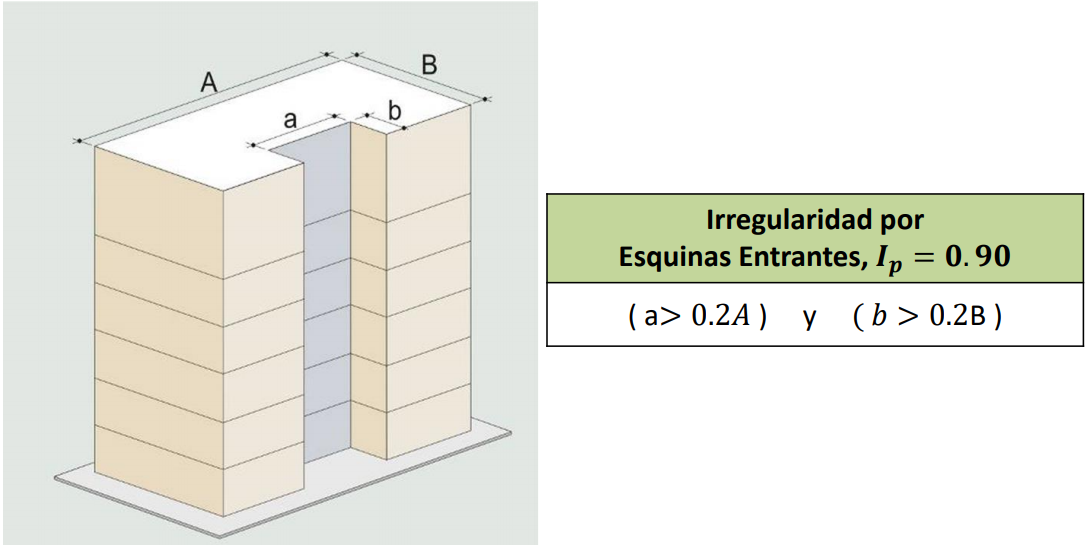
\includegraphics[scale=0.5]{images/i_esquinas.PNG}%
\caption*{\small Fuente: Muñoz (2020)}%
\end{figure}

%


\begin{table}[H]%
\centering%
\caption{Irregularidad por esquinas entrantes}%
\begin{tabular}{llcr}%
\cline{1-3}%
\multicolumn{2}{l}{Esquina entrante en X(a)} & 4.95 & \multicolumn{1}{l}{m} \\%
\multicolumn{2}{l}{Esquina entrante en Y(b)} & 2.3 & \multicolumn{1}{l}{m} \\%
\multicolumn{2}{l}{Dimensión total en X(A)} & 7.51 & \multicolumn{1}{l}{m} \\%
\multicolumn{2}{l}{Dimensión total en Y(B)} & 15.28 & \multicolumn{1}{l}{m} \\%
\multicolumn{2}{l}{a/A} & 65.91 & \multicolumn{1}{l}{\%} \\%
\multicolumn{2}{l}{b/B} & 15.05 & \multicolumn{1}{l}{\%} \\%
\multicolumn{2}{l}{Limite <} & 20.0 & \multicolumn{1}{l}{\%} \\%
\multicolumn{2}{l}{Verificación} & \textcolor[rgb]{ .267,  .447,  .769}{\textbf{Regular}} & \multicolumn{1}{l}{} \\%
\cline{1-3}%
\end{tabular}%
\end{table}

%
\subsection{Análisis Dinámico Espectral Art. 29 E{-}030}%
\label{subsec:AnlisisDinmicoEspectralArt.29E{-}030}%
El análisis dinámico modal espectral consiste calcular la respuesta para cada modo ingresando al espectro de pseudo-aceleraciones definido en \ref{ssubsec:Espectroderespuestadeaceleraciones}, para posteriormente combinar los resultados según los criterios que se menciona en la norma E-030:%
%insertion

%
\subsubsection{Criterios de combinación}%
\label{ssubsec:Criteriosdecombinacin}%
%insertion%
\begin{tcolorbox}[colback=gray!5!white,colframe=Maroon!75!black,fonttitle=\bfseries,title=Art. 29.3.1]%
\textit{Mediante los criterios de combinación que se indican, se puede obtener la respuesta máxima elástica esperada (r) tanto para las fuerzas internas en los elementos componentes de la estructura, como para los parámetros globales  del edificio como fuerza cortante en la base, cortantes de entrepiso, momentos  de volteo, desplazamientos totales y relativos de entrepiso.}%
\end{tcolorbox}%
\begin{tcolorbox}[colback=gray!5!white,colframe=Maroon!75!black,fonttitle=\bfseries,title=Art. 29.3.2]%
\textit{La respuesta máxima elástica esperada (r) correspondiente al efecto conjunto  de  los  diferentes  modos  de  vibración  empleados  (ri)  puede determinarse usando la combinación cuadrática completa de los valores calculados para cada modo.}%
\end{tcolorbox}%
\begin{alignat}{1}%
r=\sqrt{\sum \sum r_{i}\,\rho _{ij}\,r_{j}}%
\end{alignat}%
\begin{tcolorbox}[colback=gray!5!white,colframe=Maroon!75!black,fonttitle=\bfseries,title=Art. 29.3.3]%
\textit{Donde r representa las respuestas modales, desplazamientos o fuerzas, los coeficientes de correlación están dados por:}%
\end{tcolorbox}%
\begin{alignat}{1}%
\rho_{ij}=\frac{8\beta ^{2}\left ( 1+\lambda  \right )\lambda ^{3/2}}{\left ( 1-\lambda ^{2} \right )+4\beta ^{2}\lambda \left ( 1+\lambda  \right )^{2}}\quad\quad  \lambda =\frac{\omega _{j}}{\omega _{i}}%
\end{alignat}%
\begin{flushleft}%
Donde:\\%
$\beta$: fracción del amortiguamiento crítico, que se puede suponer constante para todos los modos igual a 0,05.\\%
$\omega _{j}$,$\omega _{i}$: son las frecuencias angulares de los modos i, j\\%
\end{flushleft}

%
\subsection{Determinación de desplazamientos laterales Art. 31 E{-}030}%
\label{subsec:DeterminacindedesplazamientoslateralesArt.31E{-}030}%
%insertion%
\begin{tcolorbox}[colback=gray!5!white,colframe=Maroon!75!black,fonttitle=\bfseries,title=Art. 31.3.1]%
\textit{Para  estructuras  regulares, los  desplazamientos  laterales  se  calculan multiplicando por 0,75 R los resultados obtenidos del análisis lineal y elástico con las solicitaciones sísmicas reducidas. Para estructuras irregulares, los desplazamientos laterales se calculan multiplicando por 0,85 R los resultados obtenidos del análisis lineal elástico.}%
\end{tcolorbox}%


\begin{figure}[H]%
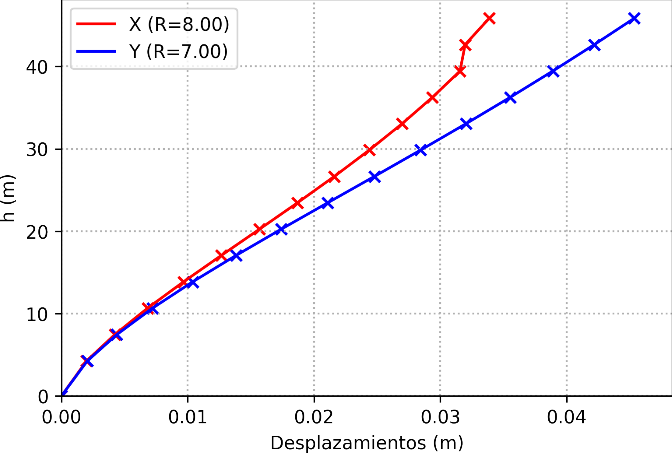
\includegraphics[width=0.8\textwidth]{images/desplazamientos_laterales}%
\caption{Desplazamientos inelásticos}%
\end{figure}

%
\subsection{Verificación de derivas máximas Art. 32 E{-}030}%
\label{subsec:VerificacindederivasmximasArt.32E{-}030}%
%insertion%


\begin{table}[ht!]%
\centering%
\caption{Derivas máximas}%
\begin{tabular}{>{\raggedright\arraybackslash}p{9.8cm} >{\raggedleft\arraybackslash}p{1cm}}%
\hline%
\multicolumn{2}{c}{\multirow{2}[1]{*}{\textbf{LIMITES PARA LA DISTORSION DE ENTREPISO}}} \\%
\multicolumn{2}{c}{} \\%
\hline%
\textbf{Material predominante:} & $\Delta_{i}/h_{ei}$ \\%
\hline%
{Concreto Armado\cellcolor[rgb]{ .949,  .949,  .949} } & \textcolor[rgb]{ 1,  0,  0}{\textbf{0.007}}\cellcolor[rgb]{ .949,  .949,  .949} \\%
\hline%
{Acero} & 0.01 \\%
\hline%
{Albañilería} & 0.005 \\%
\hline%
{Madera} & 0.01 \\%
\hline%
{Edificios de concreto armado con muros de ductilidad limitada} & 0.005 \\%
\hline%
\end{tabular}%
\caption*{Fuente: E-030 (2018)}%
\end{table}

%


\begin{figure}[ht!]%
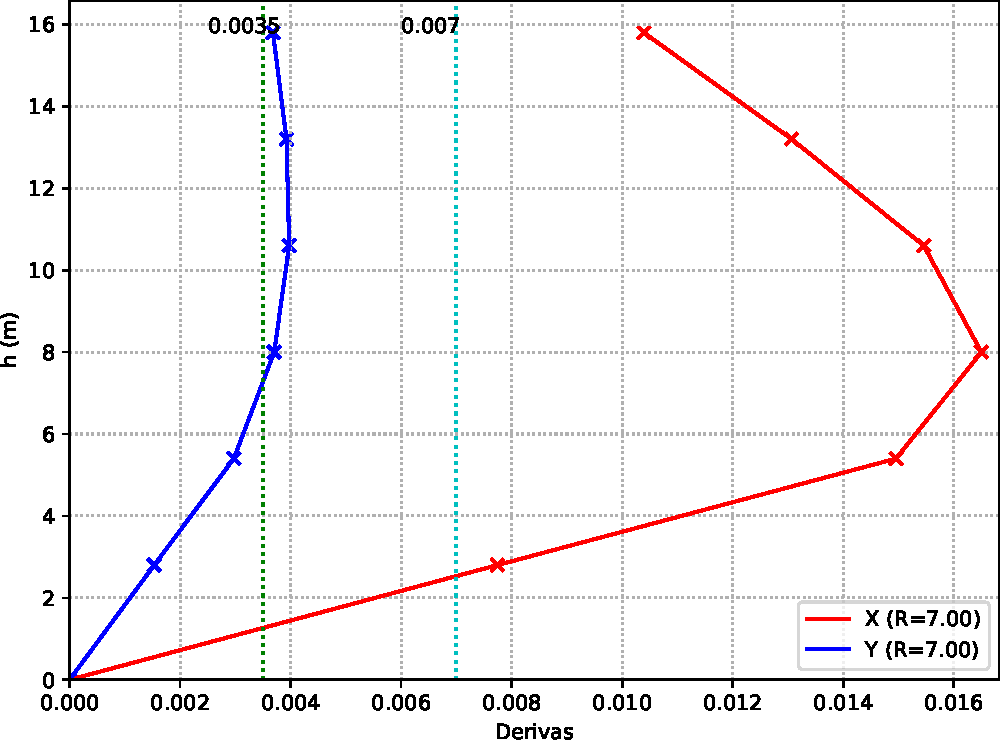
\includegraphics[width=0.8\textwidth]{images/derivas}%
\caption{Derivas máxima de entrepiso}%
\end{figure}

%
\subsection{Verificación del sistema estructural}%
\label{subsec:Verificacindelsistemaestructural}%
Se verificará que efectivamente se tiene un sistema estructural de muros en la dirección X, en la dirección Y no se verificara dado que no existen muros estructurales. Como se muestra en la figura \ref{fig:sist_est_etabs} el valor de cortante que absorben los muros es de 64 ton, y la cortante total es aproximadamente 70 ton (ver figura \ref{fig:corte_basal}) por lo que el porcentaje que toman los muros es mayor al 90\%.%
%insertion%


\begin{figure}[ht!]%
\centering%
\caption{Sistema estructural}%
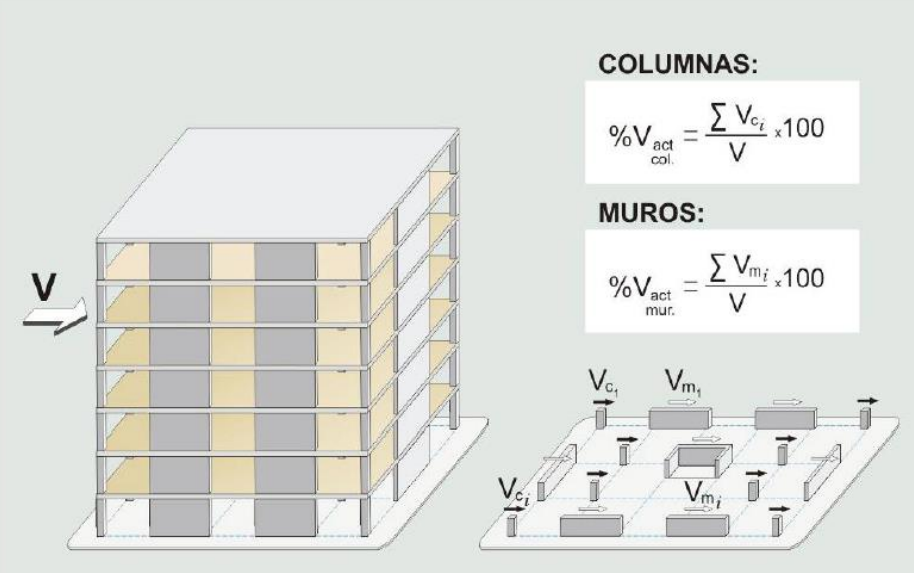
\includegraphics[scale=0.7]{images/sist_estructural.PNG}%
\caption*{\small Fuente: Muñoz (2020)}%
\label{fig:sist_est}%
\end{figure}

%


\begin{figure}[ht!]%
\centering%
\caption{Verificación del sistema estructural en X}%
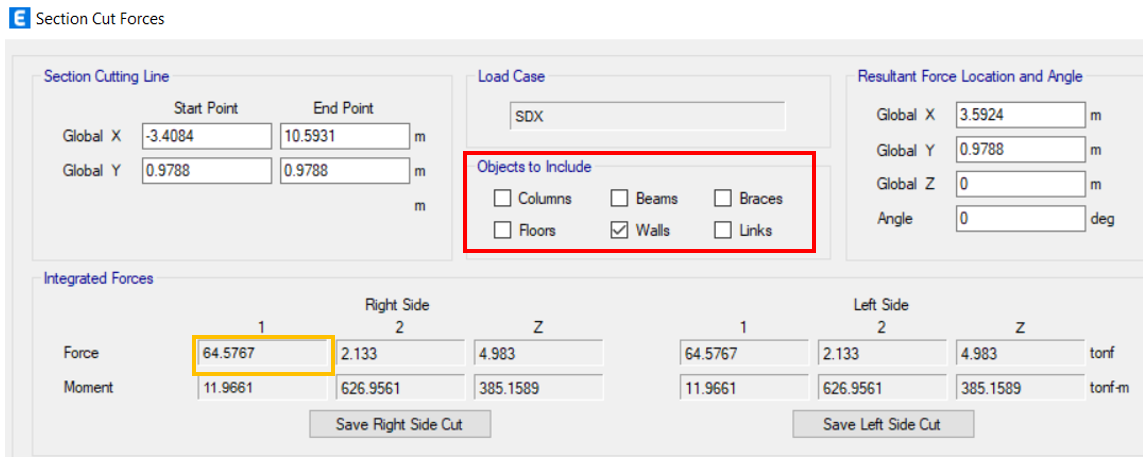
\includegraphics[scale=0.7]{images/sist_estructural_etabs.PNG}%
\caption*{\small Fuente: Muñoz (2020)}%
\label{fig:sist_est_etabs}%
\end{figure}

%
\subsection{Análisis estático o de fuerzas estáticas equivalentes Art. 28 E{-}030}%
\label{subsec:AnlisisestticoodefuerzasestticasequivalentesArt.28E{-}030}%
%insertion

%
\subsubsection{Fuerza cortante en la base Art 28.2 E{-}030}%
\label{ssubsec:FuerzacortanteenlabaseArt28.2E{-}030}%
%insertion%
\begin{tcolorbox}[colback=gray!5!white,colframe=Maroon!75!black,fonttitle=\bfseries,title=Art. 28.2.1]%
\textit{La fuerza cortante total en la base de la estructura, correspondiente a la dirección considerada, se determina por la siguiente expresión:}%
\end{tcolorbox}%
\begin{alignat}{1}%
V=\frac{Z\;\cdot U\cdot\;C\cdot\;S}{R}\;P\;\;\;\;\;\;\;\;\;\;\;\frac{C}{R}\geq 0,11%
\end{alignat}%
Según el articulo 28.4.2 el periodo fundamental de vibración puede estimarse con la ecuación:%
\begin{alignat}{1}%
T=2\pi\cdot \displaystyle\sqrt{\frac{\left (\displaystyle\sum_{i=1}^{n} P_{i}\cdot d_{i}^{2}\right )}{g\cdot\left (\displaystyle\sum_{i=1}^{n}f_{i}\cdot d_{i}  \right ) }}%
\end{alignat}%
\begin{flushleft}%
Donde:\\%
$P_{i}$: es el peso sísmico en el nivel i.\\%
$f_{i}$: es la fuerza lateral en el nivel i correspondiente a una distribución en altura semejante a la del primer modo en la dirección de análisis.\\%
$d_{i}$: es el desplazamiento lateral del centro de masa del nivel  i en traslación pura (restringiendo los giros en planta) debido a las fuerzas $f_{i}$. Los desplazamientos se calculan suponiendo comportamiento lineal elástico de la estructura y, para el caso de estructuras de concreto armado y de albañilería, considerando las secciones sin fisurar.\\%
\end{flushleft}%
Lo anterior equivale a calcular los modos de vibrar en el modelo matemático restringiendo el grado de libertad de rotación.Lo anterior equivale a calcular los modos de vibrar en el modelo matemático restringiendo el grado de libertad de rotación.%


\begin{figure}[ht!]%
\centering%
\subfigure[X]{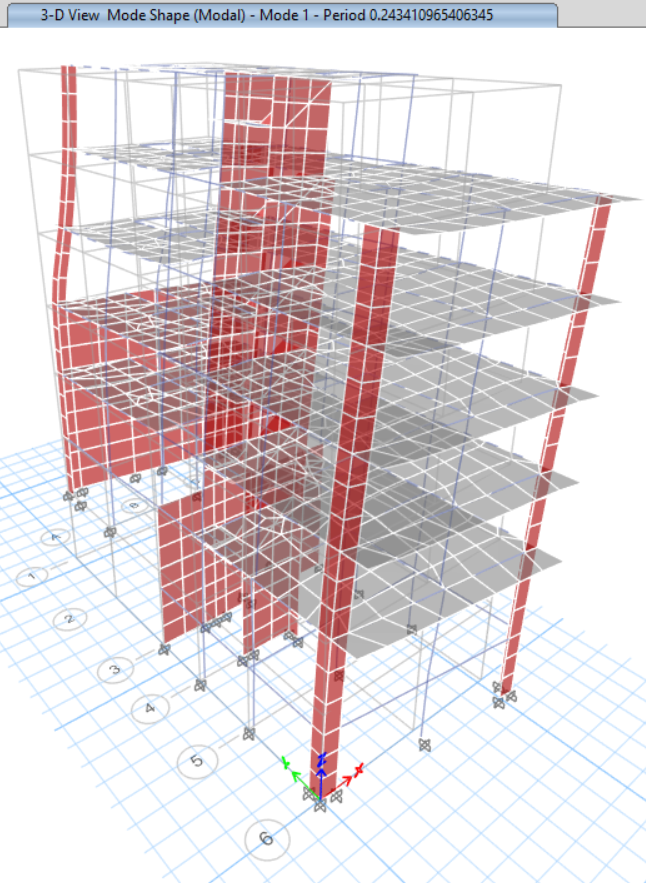
\includegraphics[height=70mm]{images/TX.PNG}}\hspace{1cm}%
\subfigure[Y]{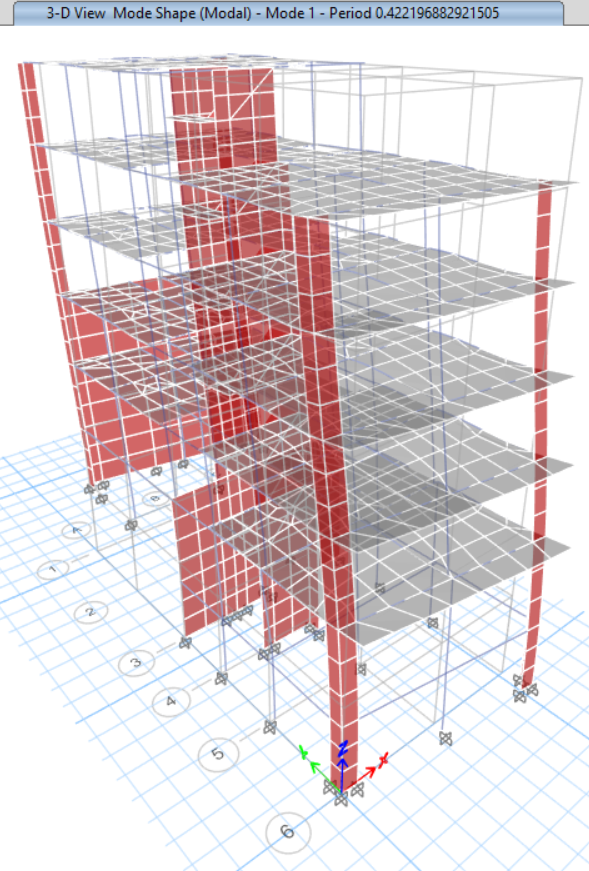
\includegraphics[height=70mm]{images/TY.PNG}}%
\caption{Periodos fundamentales en traslación pura}%
\label{fig:periodos_fund}%
\end{figure}

%


\begin{table}[H]%
\centering%
\caption{Análisis sísmico estático}%
\extrarowheight = 0ex%
\renewcommand{\arraystretch}{1.2}%
\begin{tabular}{>{\arraybackslash}m{7cm}|>{\centering\arraybackslash}m{2.5cm}|>{\centering\arraybackslash}m{2cm}|>{\centering\arraybackslash}m{2cm}|}%
\cline{2%
-%
4}%
&\multicolumn{3}{c|}{\textbf{PARÁMETROS SÍSMICOS}}\\%
\cline{2%
-%
4}%
&&\textit{\textbf{X}}&\textit{\textbf{Y}}\\%
\cline{2%
-%
4}%
\textit{Factor de Zona (Tabla N° 1)}&\textbf{Z}&\multicolumn{2}{c|}{0.45}\\%
\cline{2%
-%
4}%
\textit{Factor de Uso (Tabla N° 5)}&\textbf{U}&\multicolumn{2}{c|}{1.50}\\%
\cline{2%
-%
4}%
\textit{Periodos en traslación pura obtenidos del ETABS (Art. 28.4.2)}&\textbf{T}&0.84&1.04\\%
\cline{2%
-%
4}%
\textit{Factor de Amplificación (Art. 14)}&\textbf{C}&1.79&1.44\\%
\cline{2%
-%
4}%
\textit{Factor de Suelo (Tabla N°3)}&\textbf{S}&\multicolumn{2}{c|}{1.05}\\%
\cline{2%
-%
4}%
\textit{Coef. Básico de Reducción (Tabla N°7)}&\textbf{R\raisebox{-0.5ex}{\scriptsize{o}}}&8.00&7.00\\%
\cline{2%
-%
4}%
\textit{Irregularidad en altura (Tabla N°8)}&\textbf{I\raisebox{-0.5ex}{\scriptsize{a}}}&1.00&1.00\\%
\cline{2%
-%
4}%
\textit{Irregularidad en planta (Tabla N°9)}&\textbf{I\raisebox{-0.5ex}{\scriptsize{p}}}&1.00&1.00\\%
\cline{2%
-%
4}%
\textit{Coef. de Reducción (Articulo 22)}&\textbf{R}&8.00&7.00\\%
\cline{2%
-%
4}%
\textit{Verificación (Articulo 28.2.2)}&\textbf{C/R>0.11}&0.22&0.21\\%
\cline{2%
-%
4}%
\textit{Peso sísmico (ETABS)}&\textbf{Ps (Ton)}&\multicolumn{2}{c|}{14044.93}\\%
\cline{2%
-%
4}%
\textit{Coeficientes}&\textbf{ZUCS/R}&0.16&0.15\\%
\cline{2%
-%
4}%
\textit{Cortante estática (Art.28.2)}&\textbf{V (ton)}&\cellcolor[rgb]{ 1,  .949,  .8}\textcolor[rgb]{ 1,  0,  0}{\textbf{2232.58}}&\cellcolor[rgb]{ 1,  .949,  .8}\textcolor[rgb]{ 1,  0,  0}{\textbf{2049.06}}\\%
\cline{2%
-%
4}%
\textit{Coeficiente k (Art.28.3.2)}&\textbf{k}&1.17&1.27\\%
\cline{2%
-%
4}%
\end{tabular}%
\end{table}

%


\begin{table}[H]%
\centering%
\caption{Análisis sísmico estático por pisos}%
\begin{tabular}{ccccccccccc}
\toprule
Piso & Peso & Altura & $H^{kx}$ & $H^{ky}$ & PxHx & PxHy & ax & ay & Vx & Vy \\
\midrule
CM & 29.015 & 58.050 & 114.850 & 174.140 & 3332.293 & 5052.809 & 0.005 & 0.003 & 10.453 & 6.675 \\
TECHO 14 & 317.437 & 55.450 & 108.860 & 164.300 & 34556.903 & 52153.651 & 0.049 & 0.034 & 108.400 & 69.223 \\
TECHO 13 & 509.791 & 52.250 & 101.560 & 152.350 & 51774.624 & 77664.186 & 0.073 & 0.051 & 162.410 & 103.713 \\
TECHO 12 & 843.949 & 49.050 & 94.330 & 140.590 & 79612.774 & 118651.507 & 0.112 & 0.078 & 249.734 & 159.477 \\
TECHO 11 & 875.013 & 45.850 & 87.190 & 129.040 & 76288.454 & 112913.558 & 0.107 & 0.075 & 239.306 & 152.818 \\
TECHO 10 & 875.013 & 42.650 & 80.120 & 117.710 & 70106.760 & 102997.480 & 0.099 & 0.069 & 219.915 & 140.435 \\
TECHO 09 & 875.013 & 39.450 & 73.140 & 106.610 & 64002.563 & 93280.784 & 0.090 & 0.063 & 200.767 & 128.207 \\
TECHO 08 & 875.013 & 36.250 & 66.260 & 95.740 & 57981.069 & 83775.165 & 0.081 & 0.057 & 181.879 & 116.145 \\
TECHO 07 & 875.013 & 33.050 & 59.480 & 85.130 & 52048.322 & 74494.088 & 0.073 & 0.051 & 163.268 & 104.261 \\
TECHO 06 & 875.013 & 29.850 & 52.810 & 74.800 & 46211.434 & 65453.254 & 0.065 & 0.045 & 144.959 & 92.569 \\
TECHO 05 & 875.013 & 26.650 & 46.260 & 64.770 & 40478.910 & 56671.247 & 0.057 & 0.040 & 126.977 & 81.086 \\
TECHO 04 & 870.929 & 23.450 & 39.840 & 55.050 & 34698.428 & 47945.675 & 0.049 & 0.034 & 108.844 & 69.506 \\
TECHO 03 & 875.013 & 20.250 & 33.570 & 45.690 & 29371.011 & 39978.589 & 0.041 & 0.029 & 92.133 & 58.835 \\
TECHO 02 & 875.013 & 17.050 & 27.460 & 36.720 & 24025.285 & 32130.708 & 0.034 & 0.023 & 75.364 & 48.126 \\
TECHO 01 & 914.873 & 13.850 & 21.540 & 28.200 & 19704.886 & 25797.198 & 0.028 & 0.019 & 61.811 & 39.472 \\
SEMISOTANO & 1223.668 & 9.600 & 14.040 & 17.700 & 17177.363 & 21659.045 & 0.024 & 0.017 & 53.883 & 34.409 \\
SOTANO & 1460.154 & 5.350 & 7.090 & 8.420 & 10354.183 & 12296.233 & 0.015 & 0.010 & 32.480 & 20.741 \\
\bottomrule
\end{tabular}
%
\end{table}

%
\subsection{Fuerza cortante mínima Art. 29.4 E{-}030}%
\label{subsec:FuerzacortantemnimaArt.29.4E{-}030}%
\begin{tcolorbox}[colback=gray!5!white,colframe=cyan!75!black,fonttitle=\bfseries,title=Art. 29.4.1]%
\textit{Para cada una de las direcciones consideradas en el análisis, la fuerza cortante en el primer entrepiso del edificio no puede ser menor que el 80\% del valor calculado según el artículo 25 para estructuras regulares, ni menor que el 90\% para estructuras irregulares.}%
\end{tcolorbox}%
\begin{tcolorbox}[colback=gray!5!white,colframe=cyan!75!black,fonttitle=\bfseries,title=Art. 29.4.2]%
\textit{Si fuera necesario incrementar el cortante para cumplir los mínimos señalados,  se escalan proporcionalmente todos los otros resultados obtenidos, excepto los  desplazamientos.}%
\end{tcolorbox}%
%insertion%


\begin{figure}[ht!]%
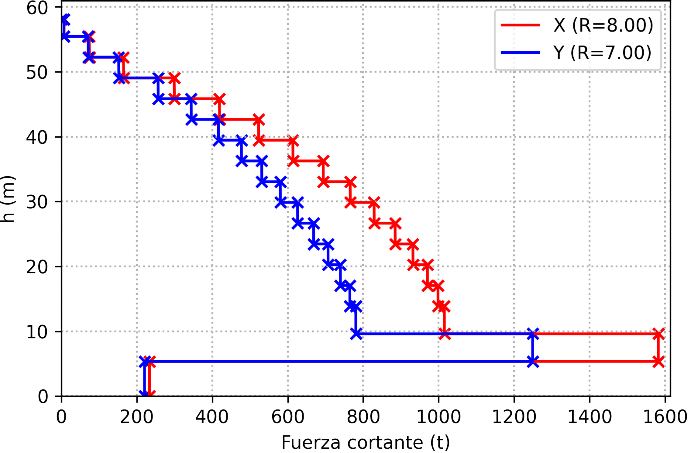
\includegraphics[width=0.8\textwidth]{images/cortantes}%
\caption{Cortantes de Entrepiso del Análisis Modal Espectral}%
\label{fig:corte_basal}%
\end{figure}

%
%insertion%


\begin{table}[H]%
\centering%
\caption{Escalamiento de la cortante dinámica}%
\begin{tabular}{ccc}
\toprule
 & X & Y \\
\midrule
V din (Ton) & 1015.25 & 780.53 \\
V est (Ton) & -1048.72 & -642.87 \\
\% min & 80.00 & 80.00 \\
\% & 96.81 & 121.41 \\
F.E. & 1.00 & 1.00 \\
\bottomrule
\end{tabular}
%
\end{table}

%
\subsection{Separación entre edificios Art. 33 E{-}030}%
\label{subsec:SeparacinentreedificiosArt.33E{-}030}%
%insertion%
\begin{tcolorbox}[colback=gray!5!white,colframe=cyan!75!black,fonttitle=\bfseries,title=Art. 33.1]%
\textit{Toda estructura está separada de las estructuras vecinas, desde el nivel del terreno natural, una distancia mínima s para evitar el contacto durante un movimiento sísmico.}%
\end{tcolorbox}%
\begin{tcolorbox}[colback=gray!5!white,colframe=cyan!75!black,fonttitle=\bfseries,title=Art. 33.2]%
\textit{Esta distancia no es menor que los 2/3 de la suma de los desplazamientos máximos de los edificios adyacentes ni menor que:}%
\end{tcolorbox}%
\begin{alignat}{1}%
s=0.006\;h\geq0.03\;m%
\end{alignat}%
Donde h es la altura medida desde el nivel del terreno natural hasta el nivel considerado para evaluar s%
\begin{tcolorbox}[colback=gray!5!white,colframe=cyan!75!black,fonttitle=\bfseries,title=Art. 33.3]%
\textit{El edificio se retira de los límites de propiedad adyacentes a otros lotes edificables,  o  con  edificaciones,  distancias  no  menores  que  2/3  del desplazamiento máximo calculado según el artículo 28 ni menores que s/2 si la edificación existente cuenta con una junta sísmica reglamentaria.}%
\end{tcolorbox}%


\begin{figure}[H]%
\centering%
\caption{Separación entre edificios}%
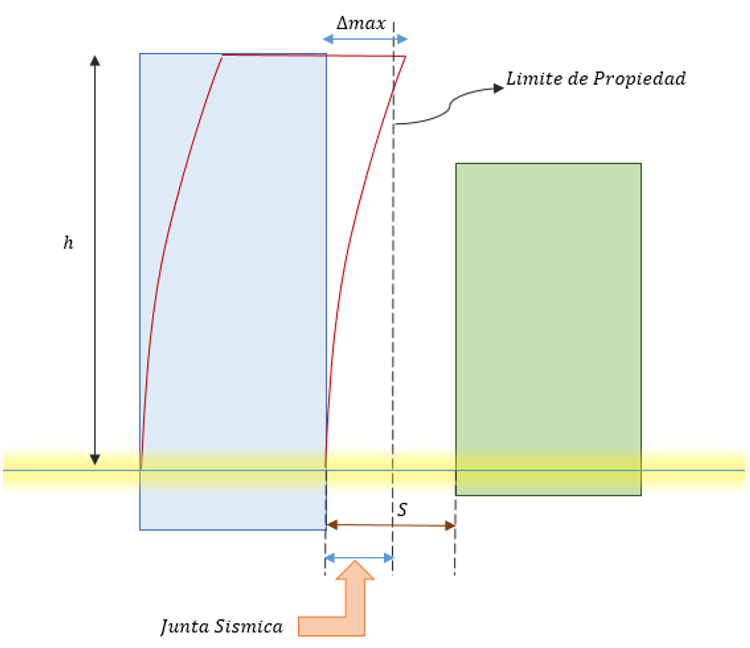
\includegraphics[scale=0.5]{images/sep_edificios.PNG}%
\label{fig:sep_edificios}%
\end{figure}

%


\begin{table}[H]%
\centering%
\caption{Cálculo de la junta sísmica}%
\extrarowheight = -0.3ex%
\renewcommand{\arraystretch}{1.5}%
\begin{tabular}{l|c|c|l}%
\cline{2-3}%
\textit{Altura del edificio} & \textbf{h} & {5805.000000000002} & {cm} \\%
\cline{2-3}%
\textit{Separación mínima entre edificios} & \textbf{s=0.006h} & {34.83} & {>3cm} \\%
\cline{2-3}%
\textit{Separación mínima del limite de propiedad} & \textbf{s/2} & {17.42} & {cm} \\%
\cline{2-3}%
\textit{Desplazamiento máximo en X} & \textbf{$\Delta_x$} & {3.39} & {cm} \\%
\cline{2-3}%
\textit{Desplazamiento máximo en Y} & \textbf{$\Delta_y$} & {4.54} & {cm} \\%
\cline{2-3}%
\textit{Separación del limite de propiedad X} & \textbf{2/3$\Delta_{x}$} & {2.26} & {cm} \\%
\cline{2-3}%
\textit{Separación del limite de propiedad Y} & \textbf{2/3$\Delta_{y}$} & {3.02} & {cm} \\%
\cline{2-3}%
\end{tabular}%
\label{tab:junta_sis}%
\end{table}

%
Según lo calculado en la tabla \ref{tab:junta_sis} %
 el edificio tendrá que ser separado del limite de propiedad 17.50 cm como mínimo en ambas direcciones, en el caso que no exista junta reglamentaria el edificio actual se separa del edificio existente el valor de s/2 que le corresponde, más el valor s/2 de la estructura vecina.
>>>>>>> main

%
\end{document}